\begin{appendices}
	% \chapter{Publicaciones}
	\chapter{miRNAfe: a comprehensive tool for feature extraction in microRNA prediction}
	\label{sec:mirnafe}
	En este trabajo se publicó la herramienta de extracción de características de secuencias tipo tallo-horquilla. Esta publicación corresponde con la primera
	etapa de la metodología desarrollada en al tesis.
	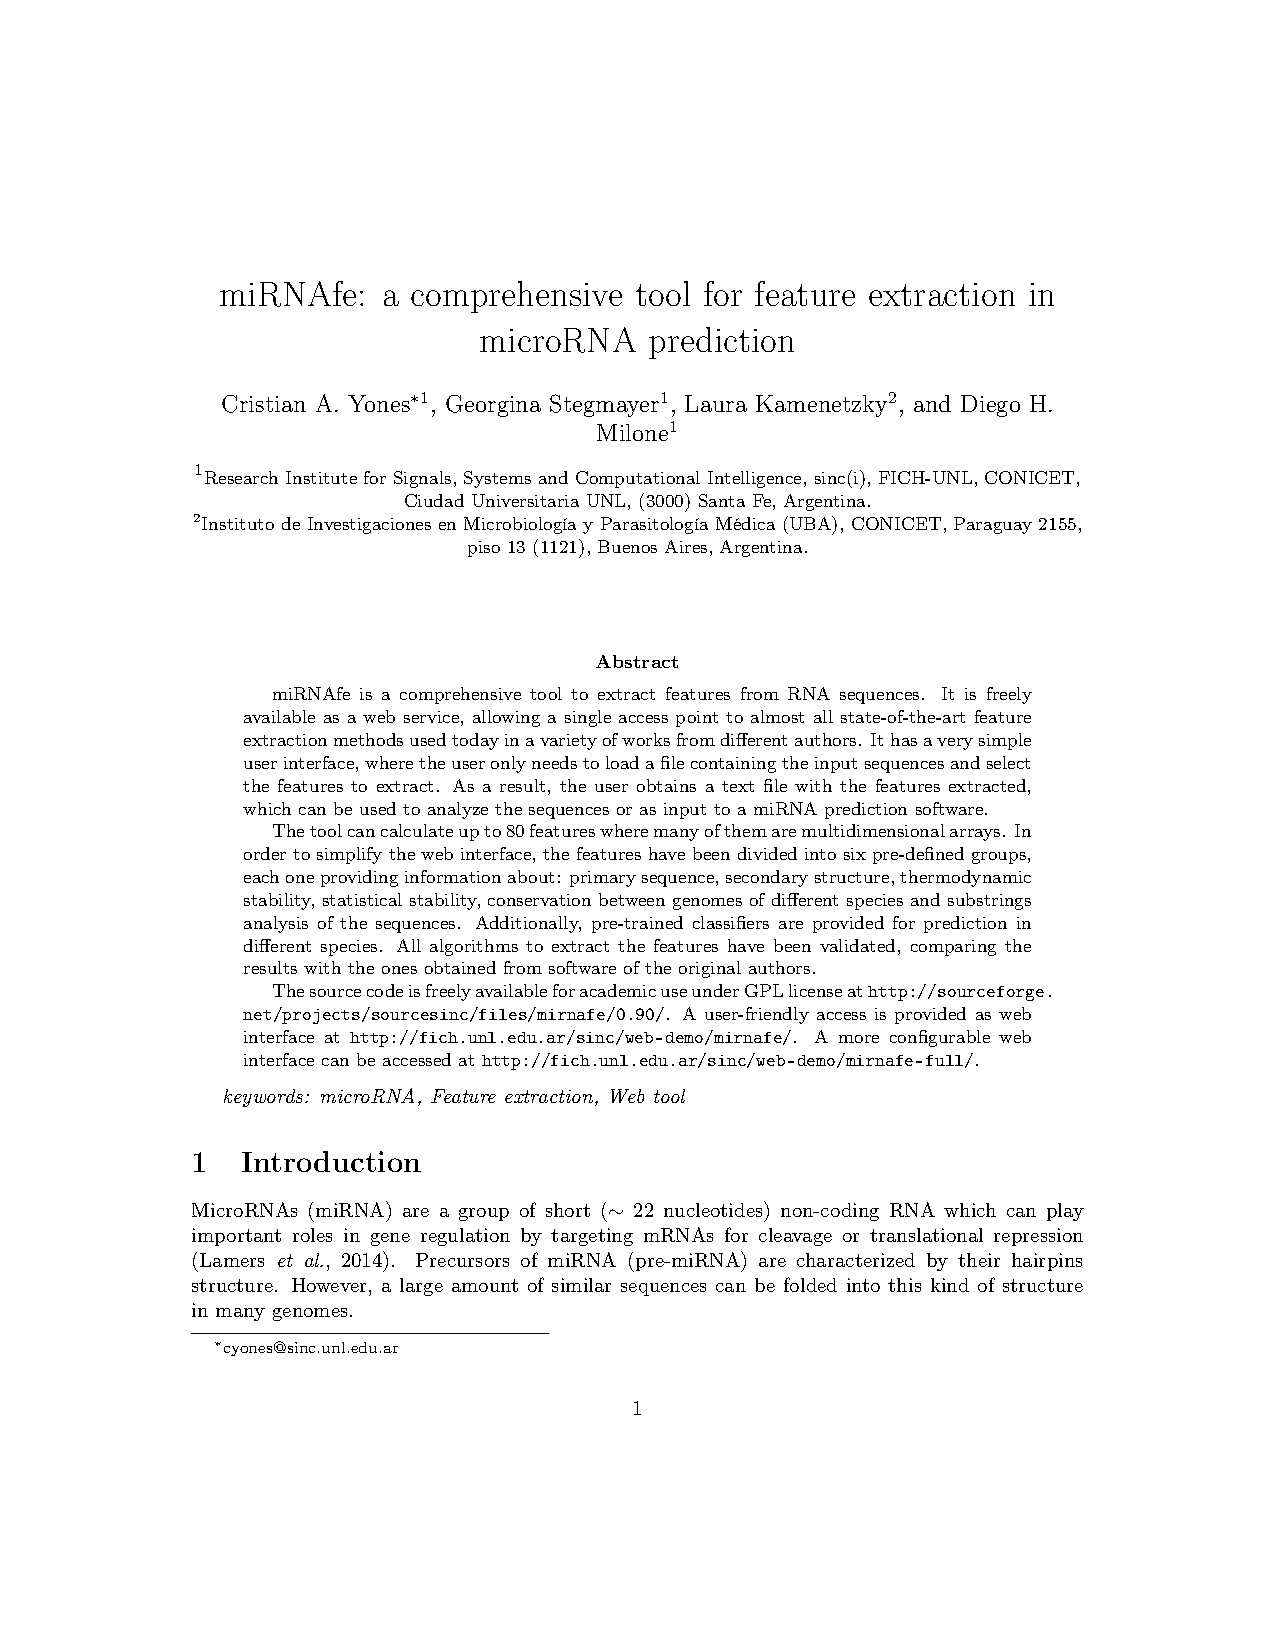
\includepdf[pages=-]{mirnafe/mirnafe.pdf}
	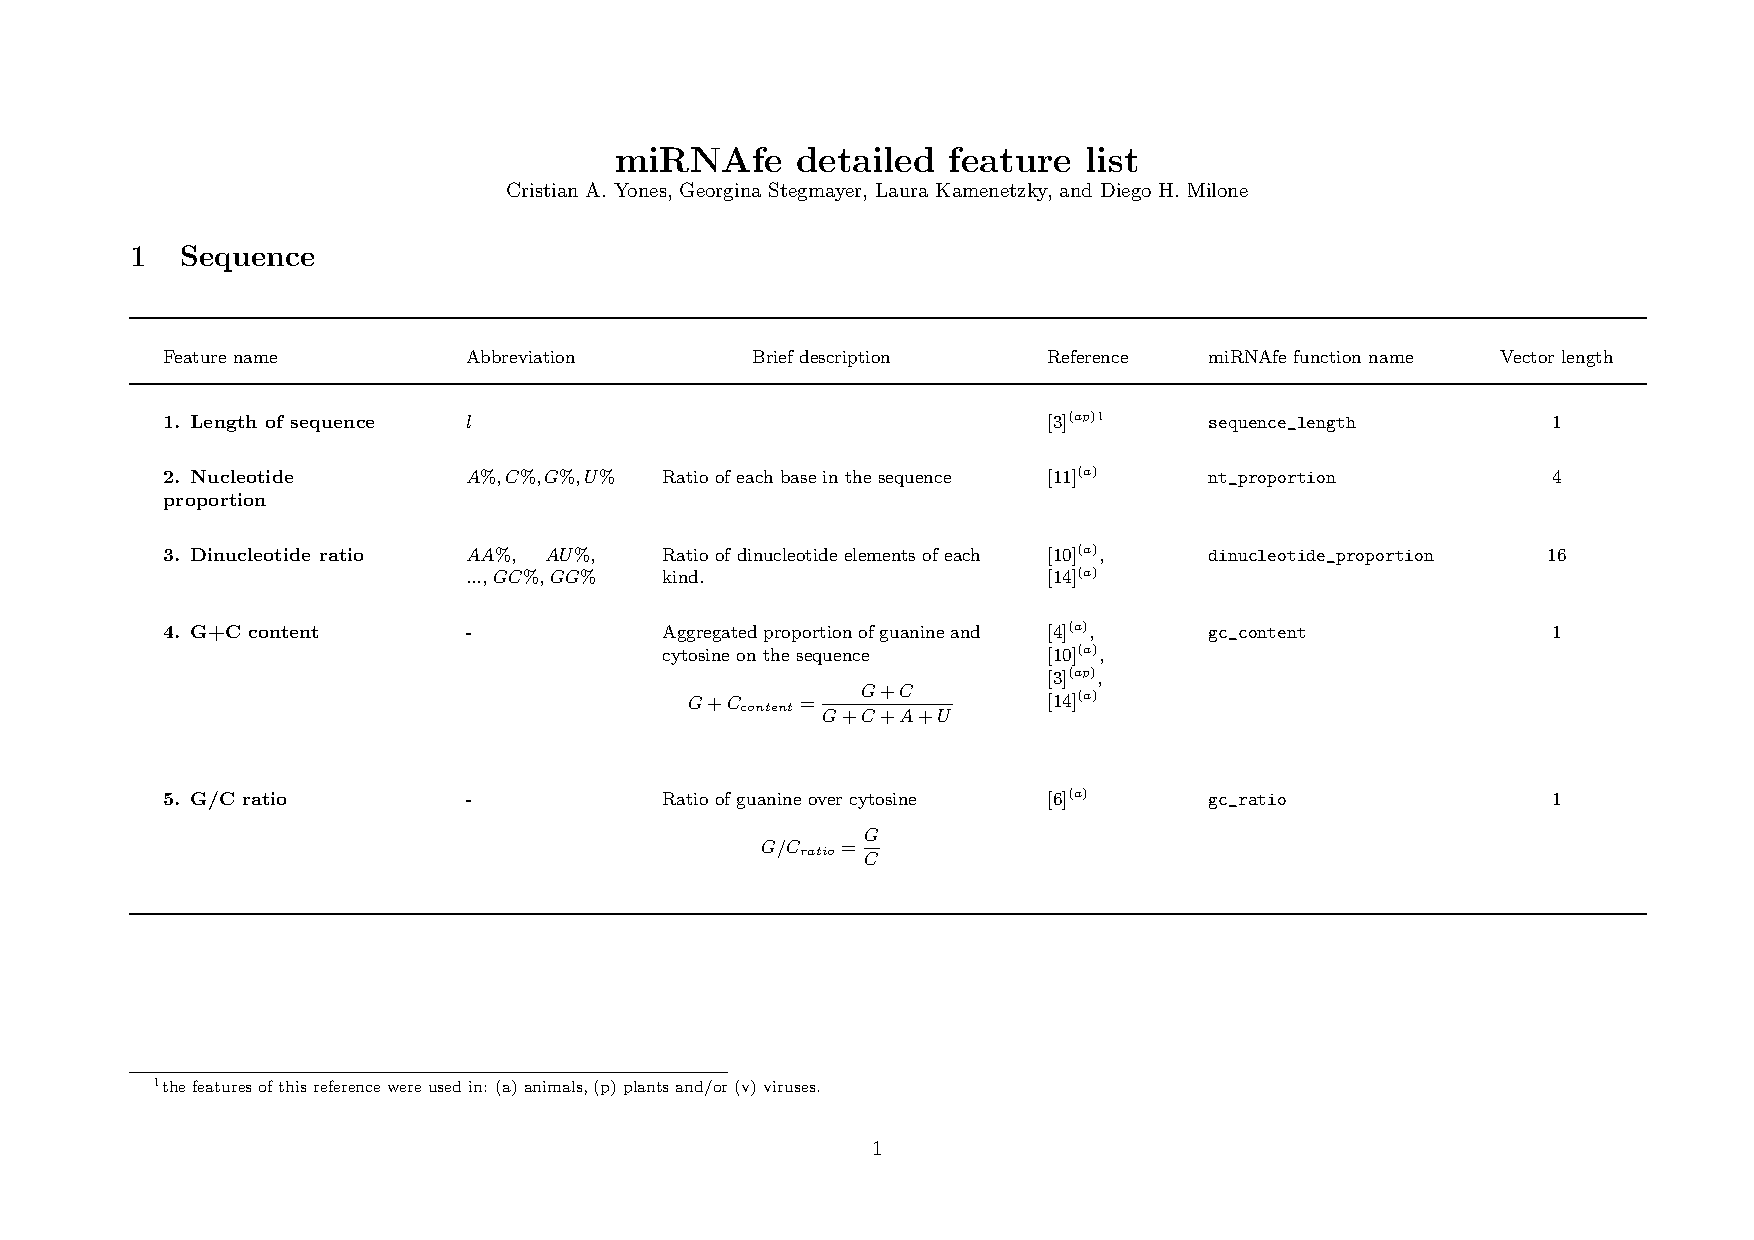
\includepdf[pages=-,angle=90]{mirnafe/supplementary_material.pdf}

	\chapter{Genome-wide pre-miRNA discovery from few labeled examples}
	\label{sec:mirnass}
	En este trabajo se presentó el metodo semi-supervisado de predicción de microRNA en genoma completo. Esta publicación corresponde con la tercera etapa de
	la metodología desarrollada en al tesis.
	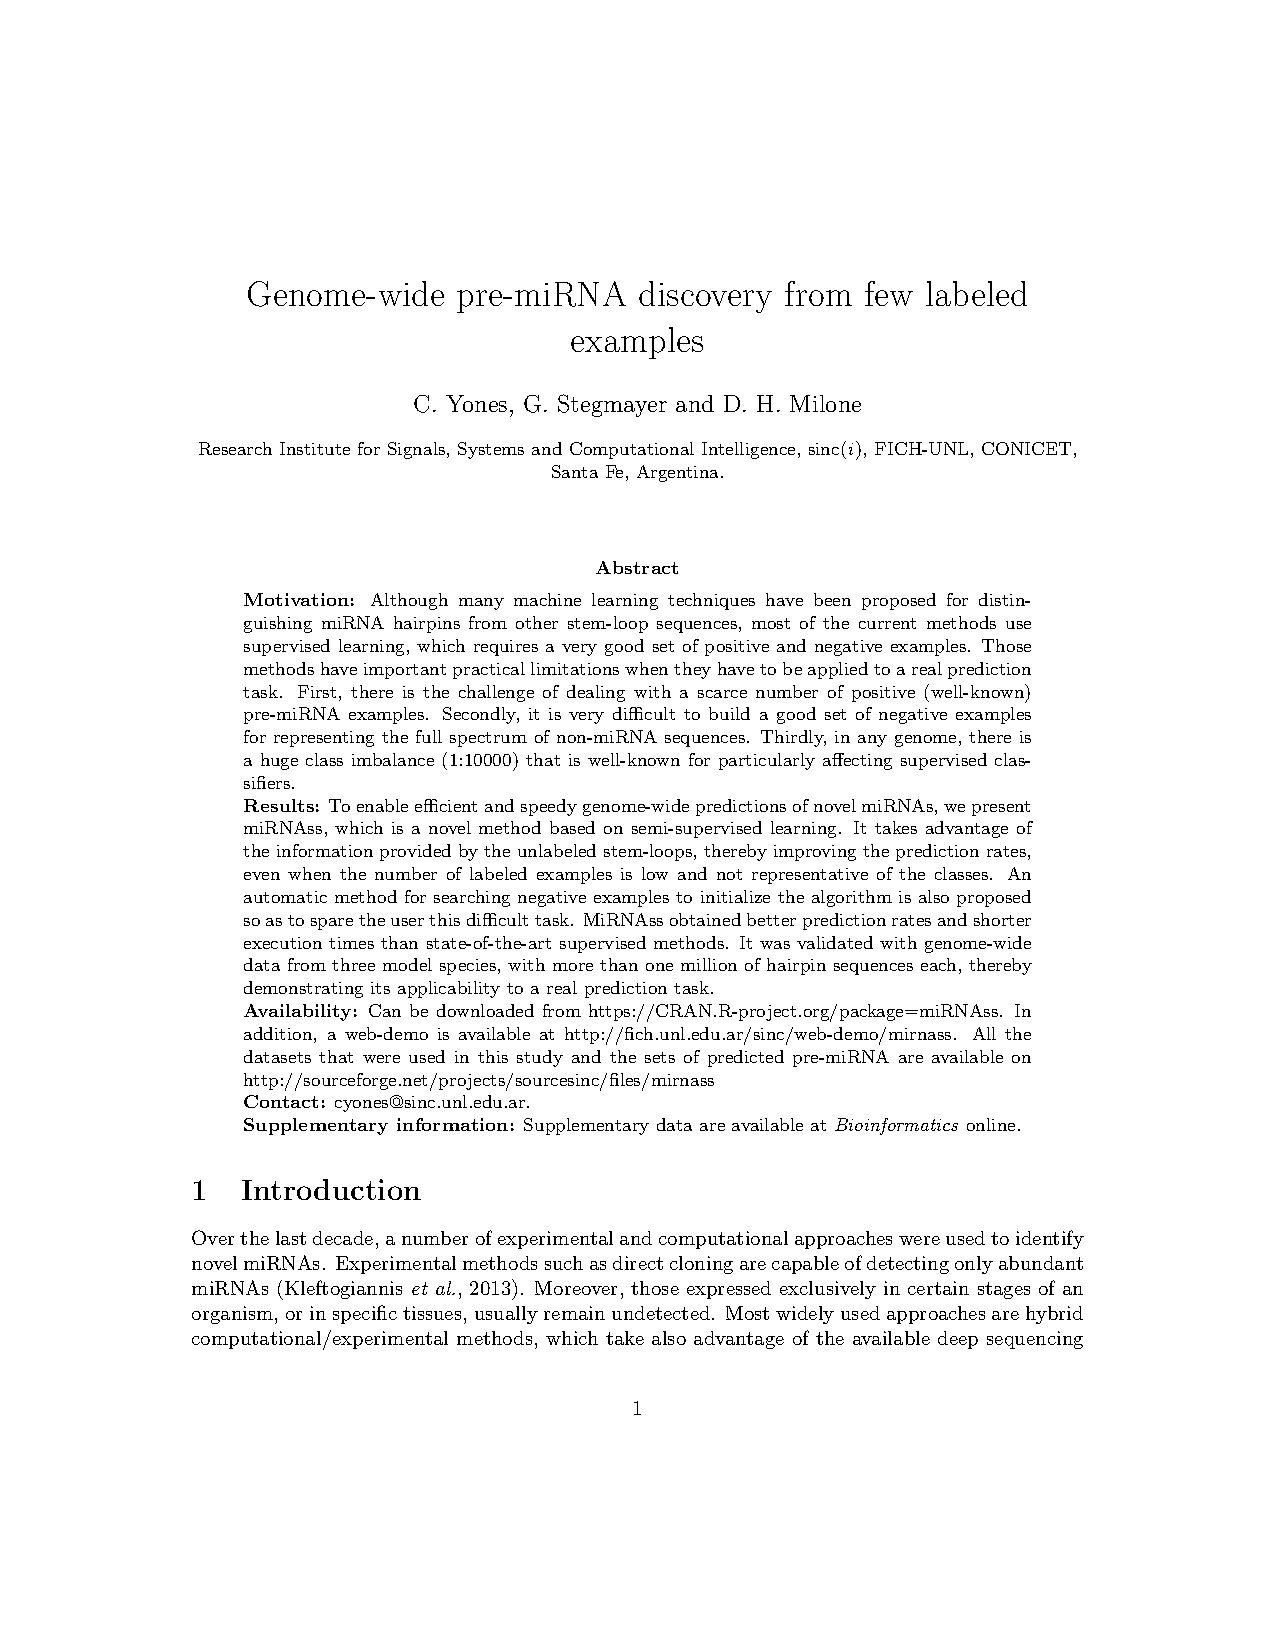
\includepdf[pages=-]{mirnass/mirnass.pdf}
	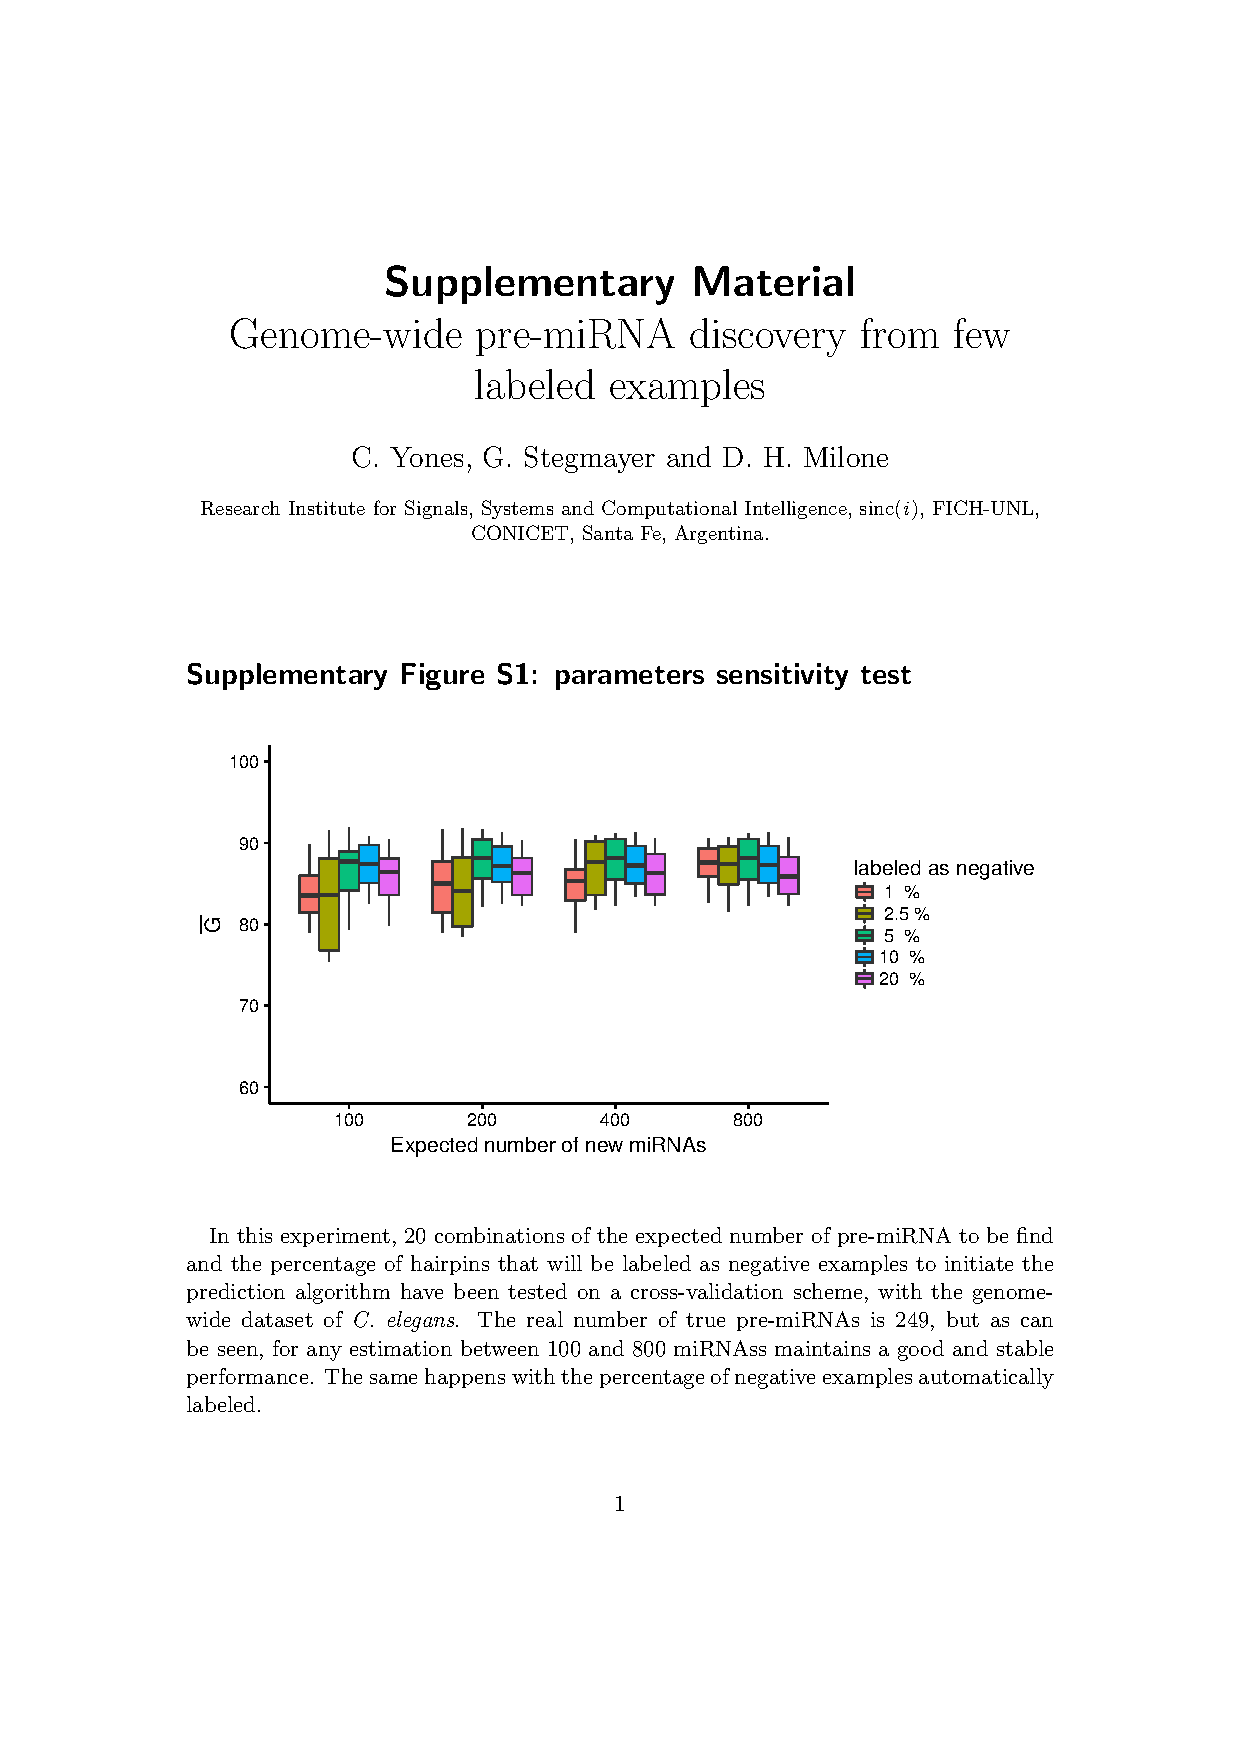
\includepdf[pages=-]{mirnass/supplementary_material.pdf}
\end{appendices}
